%% Last update: Oct. 21, 2020
\newcommand{\ignore}[1]{}

%\subsubsection{\stid{3.07} Factorization Based Sparse Solvers and Preconditioners for Exascale} \label{subsubsect:strumpack}
\subsubsection{\stid{3.07} STRUMPACK-SuperLU} \label{subsubsect:strumpack}

\paragraph{Overview} 
% \textit{Provide an overview of your project.  You might find that the introductory text from your Fall 2017 Project Summary \url{https://confluence.exascaleproject.org/display/1ST/Fall+2017+ECP+ST+Project+Summaries} useful as a starting draft.}
This project will deliver factorization-based sparse solvers
encompassing the two widely used algorithm variants: supernodal
(SuperLU: \url{https://portal.nersc.gov/project/sparse/superlu})
and multifrontal (STRUMPACK: \url{http://portal.nersc.gov/project/sparse/strumpacK}).
STRUMPACK is
further enhanced with scalable preconditioning using
hierarchical and data-sparse matrix algebra. Both libraries are purely algebraic,
applicable to many application domains. We will address
several Exascale challenges, with the following
focus areas: 
(1) Develop novel approximation algorithms that have lower
arithmetic and communication complexity with respect to the size of the
input matrix;
(2) Develop new parallelization strategies that reduce
inter-process communication and expose task parallelism and vectorization
for irregular computations involving sparse data structures to better
use on-node resources;
(3) Integrate our software into higher-level
algebraic solvers such as hypre, PETSc, Trilinos, and collaborate with
ECP teams for application-specific and hardware-specific tuning
of the parameters space to achieve optimal efficiency.

Our solver technology is essential for ECP, because many 
% DOE simulation and data analysis 
codes expected to run on Exascale machines need
solutions of sparse algebraic systems, and many high-fidelity simulations
involve large-scale multiphysics and multiscale modeling problems that
generate highly ill-conditioned and indefinite algebraic equations,
for which pure iterative methods 
% such as Krylov and multigrid, albeit readily parallelizable on large machines, 
cannot converge to the solution.
The factorization-based algorithms being developed herein
represent an important class of methods that are indispensable building
blocks for solving those numerically challenging problems. Our software
can often be used as a reliable standalone solver, or as a preconditioner
for Krylov methods, or as a coarse grid solver in multigrid
methods. %, just to name a few.

%\vspace{-10pt}
\paragraph{Key Challenges}
%\textit{Describe what is hard to do, why it is challenging.}
At Exascale we need to address several major challenges:
decreasing amount of memory per core, increasing impact of communication
cost and load imbalance, and increasing architectural heterogeneity.
Our new design of algorithms and codes must focus on
reducing communication and synchronization and task scheduling 
instead of floating point operation throughput. In sparse factorization
methods, we expect new bottlenecks in parts of the code
that previously received little attention. For example, the preprocessing
step involves numerical pivoting for selecting stable pivots and
symbolic factorization, which do not yet parallelize well on manycore
architectures with fine-grained parallelism.
At Exascale, direct solvers are more likely to
be used in a preconditioning strategy, for example, in block Jacobi
preconditioning, in domain decomposition methods or as coarse-grid
solvers in algebraic multigrid, which requires repeated triangular
solves. The challenge here is to mitigate the low arithmetic intensity
and high degree of data dependency.

Compared to iterative methods, the primary bottleneck of direct solvers
is the asymptotically higher growth in memory need and floating point
operations, especially for problems from three-dimensional geometry.
It is imperative to develop new factorization methods that require
much less memory and data movement.

%\vspace{-10pt}
\paragraph{Solution Strategy}
%\textit{Describe your basic strategy for addressing the challenges.}
We will address these challenges in several thrust areas.
The new techniques will be implemented in the two software packages SuperLU
and STRUMPACK. The former is a widely used sparse direct solver based on
supernodal factorization and the latter is a newer direct
solver/preconditioner package based on multifrontal factorization 
and hierarchical low-rank matrix structures.
% Parallel pre-pivoting for both packages.

The improvements for SuperLU will be mainly in two areas: (1) develop
the communication-avoiding 3D factorization and triangular solve
algorithms and codes that have provably lower communication complexity;
(2) develop a synchronization-avoiding triangular solve code to enable more
overlap of communications of different processes at different substitution steps;
(3) develop new multiGPU codes for both symbolic preprocessing step and
numerical factorization and solve steps.

In addition to exploiting structural sparsity as SuperLU does, STRUMPACK
also exploits data sparseness in the dense blocks of sparse factors using
low-rank representations, which leads to linear scaling $O(n)$ or $O(n \log n)$
memory and arithmetic complexity for PDEs with smooth kernels.
The developments for STRUMPACK will focus on several areas:
\ignore{ %% old
(1) develop robust stopping criteria --- both absolute and relative --- for
    adaptive (incremental) randomized sampling schemes to reveal numerical
    ranks in the low-rank compression routine. The goal is to use
    enough samples for stability, but not too many for efficiency;
(2) add OpenMP support for both HSS compression and ULV factorization routines,
    especially use OpenMP task construct to support irregular parallelism;
(3) reduce MPI communication in all stages of the code, including HSS
    construction, ULV factorization and triangular solve;
(4) in addition to HSS, develop codes to support other simpler low-rank
    formats, such as HOLDR and BLR. The HSS format has asymptotically
    lower complexity than HOLDR and BLR, but has a larger prefactor constant.
    We expect HSS to be more useful for large-scale problems while HOLDR
    and BLR are more useful for mid-range problems;
(5) work with ECP application teams to examine their specific problem
    characteristics and develop the best clustering/ordering methods to 
    reveal low-rank structures.
}
%
(1) development of an advanced preconditioner based on approximate
multifrontal LU factorization, combining small dense fronts, medium
sized Block Low-Rank (BLR) fronts (reducing the complexity pre-factor)
and large fronts compressed using the Hierarchically Off-Diagonal
Butterfly (HODBF) representation (leading to nearly linear scaling for
large high-frequency problems); (2) port the BLR algorithms --
including several variants like left and right-looking, low-rank
update and accumulate -- to GPUs (targeting CUDA, HIP/ROCm and
SYCL/DPC++), and include in the preconditioner; and
%targeting Perlmutter, Frontier and Aurora.  (3) reduce
%MPI communication
(3) develop sparse direct solvers (preconditioners) that are fully
resident on the GPU, including reordering and symbolic analysis.
%. (4)
%work with ECP application teams to examine their specific problem
%characteristics

%\vspace{-10pt}
\paragraph{Recent Progress}
%\textit{Describe what you have done recently.  It would be good to have some kind of figure or diagram in this section.}
\ignore{ %%%% replace the following by the new activities
In the past six months, we added more support for GPUs and
improved on-node threading performance.  To this end, we participated
in the 3.5-day ECP OpenMP Hackathon at NERSC in August 2019,
working closely with the HPCToolkit and SOLLVE teams,
as well as the OpenMP/vectorization experts from Intel.  
Using HPCToolkit revealed several performance bottlenecks.  We rewrote
the code to remove a few inefficiencies, and identified solution strategies
for the other bottlenecks.

We also worked with two ECP applications: MFEM electromagnetic diffusion
problems governed by high frequency indefinite Maxwell equations
(CEED Co-Design Center) and ExaSGD Miniapp2 -- sparse ACOPF matrices:
\url{https://github.com/LLNL/hiop/tree/sandbox/matrices/data/acopf_matrices}
}  %%%% ignored

We mainly focus on the multiGPU developments. For SuperLU, the new developments are
on triangular solve with one-sided communication using Nvidia's NVSHMEM and AMD's
ROCSHMEM (in design stage).
%All the experiments are performed on Summit.
% The main algorithmic challenges we have to overcome are: parallel tasks are of non-uniform size,
% load imbalance, and memory and communication bound operations.
% For STRUMPACK we improved the GPU off-loading code. We ported the
% preconditioner based on block low-rank compression to distributed
% memory systems. We developed an interface from Trilinos to STRUMPACK.
For STRUMPACK we further improved performance of the sparse direct
solver on GPUs, by reducing memory allocations. We reduced the peak
memory usage of the BLR enabled preconditioner, allowing to solve much
larger problems.
We also worked with the ECP application ExaSGD team, applying our sparse solvers to
the linear systems coming from AC optimal power flow problems. The linear systems
arising from the Interior Point optimization loops are highly ill-conditioned,
and zero-pivots are encountered during numerical factorization.
We improved both STRUMPACK and SuperLU to deal with the situation and allow the factorization
to succeed and recover the solution accuracy by iterative refinement.

The other algorithmic changes and the results are detailed below.

%\vspace{-5pt}
\subparagraph{STRUMPACK}  % {\bf (Pieter -- update the following)}

We improved the block low-rank preconditioner to drastically
  reduce the peak memory usage. This is achieved by building the BLR
  representation one single column at a time. This has allowed us to
  solve numerically challenging 3D problems up to $350^3$, using
  double precision complex arithmetic, on 64 nodes of Cori.
We implemented different BLR variants, including left-looking
  (reducing communication), and low-rank update and accumulate
  operations (reducing algorithm complexity).
In addition to NVIDIA and AMD GPU support~\cite{ghyselsSTRUMPACKGPU}, STRUMPACK now has
  experimental support for Intel GPUs through SYCL/DPC++ and the oneAPI
  standard's variable sized batched BLAS and LAPACK routines.

%\vspace{-.13in}
\begin{figure}[htb]
  \centering
  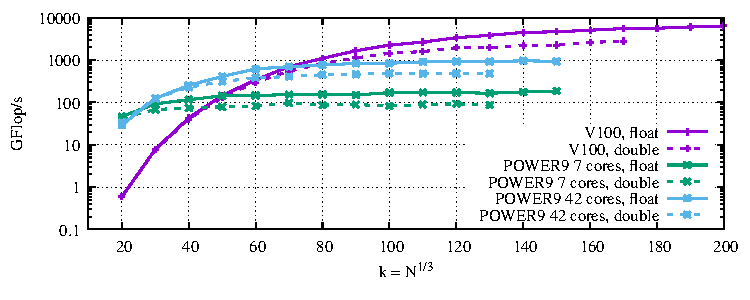
\includegraphics[scale=0.7]{projects/2.3.3-MathLibs/2.3.3.07-STRUMPACK-SuperLU/P3_V100.pdf}
 % \vspace{-.13in}
  \caption{STRUMPACK numerical factorization performance on Summit.}
  \label{fig:strumpack-parmetis-scaling}
\end{figure}

\subparagraph{SuperLU}

For the multiGPU sparse triangular solve (SpTRSV), we leverage the advantage of
  GPU-initiated data transfers of NVSHMEM.
  %  We create a novel producer-consumer paradigm to manage the computation
  % and communication in SpTRSV and implement it using two CUDA streams.
  The new  multiGPU SpTRSV implementation using two CUDA streams
  achieves a $3.7\times$ speedup when using twelve GPUs (two nodes of the Summit
  supercomputer at ORNL) relative to our implementation on a single GPU, and
  up to $6.1\times$ compared to NVIDIA's cuSOLVER (cuSPARSE csrsv2) over the range of
  one to eighteen GPUs~\cite{Sptrsv-nvshmem}.
%\item Implemented the single precision LU factorization with double precision iterative refinement.
% Initial tests show up to 50-60\% speedup on 1 node Summit using 6 CPU cores and 6 GPUs.
%  The speedup mainly comes from reduced data transfer / communication.  
In the new v7.0.0 release of SuperLU\_DIST, we released the 3D factorization algorithm,
  where MPI ranks are arranged as 3D process grid: Px X Py X Pz.  Pz direction is used
  internally for storing sub-parts of Schur-complement updates. The input \{A, B\} matrices and
  output X matrix need to reside on Px X Py. We implemented a new interface that enables
  redistribution of the users matrices between all MPI ranks and the layer Px X Py.
  The interface is flexible, allows uneven block partition of the user input, and allows separate
  calls to factorization and triangular solves.

\ignore{
\vspace{-.13in}
\begin{figure}[htb]
%\begin{minipage}[t]{0.48\columnwidth}
%% \centering
%% 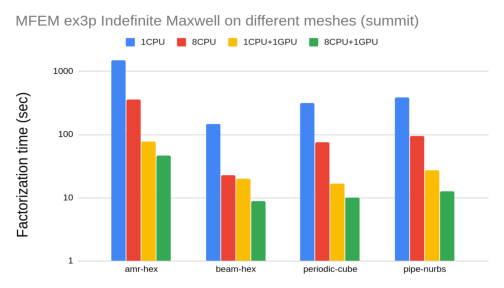
\includegraphics[scale=0.7]{projects/2.3.3-MathLibs/2.3.3.07-STRUMPACK-SuperLU/strumpack-Summit.pdf}
%% \caption{STRUMPACK factorization on Summit GPU.}
%% \label{fig:strumpack-parmetis-scaling}
%% \end{minipage}
%% \hfill
%% \begin{minipage}[t]{0.48\columnwidth}
%  \centering
% The following are for an earlier versions of CAR  
%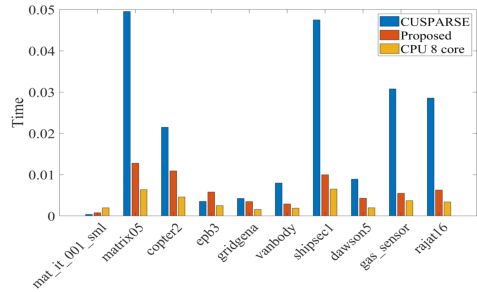
\includegraphics[scale=0.8]{projects/2.3.3-MathLibs/2.3.3.07-STRUMPACK-SuperLU/superlu-solve-Summit.pdf}
%\caption{SuperLU solve on Summit GPU.}
%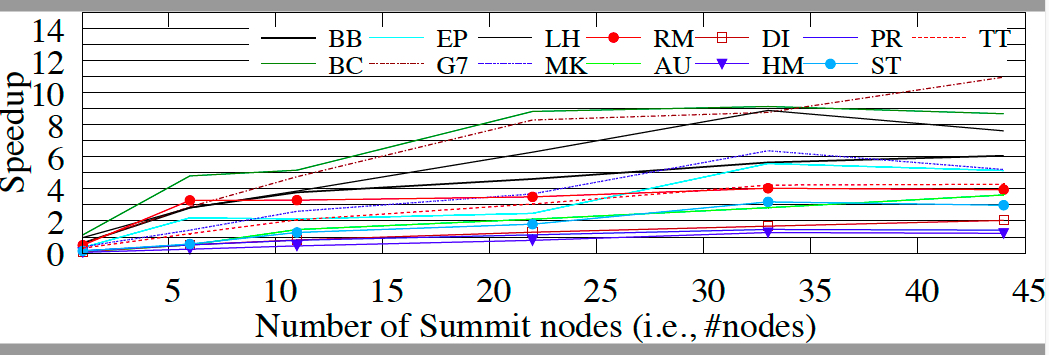
\includegraphics[scale=0.2]{projects/2.3.3-MathLibs/2.3.3.07-STRUMPACK-SuperLU/speedup_SOA.jpg}
% \caption{SuperLU symbolic factorization: GPU speedup over CPU, 13 matrices}
%  on Summit GPU nodes; 13 matrices}
%% \end{minipage}
\end{figure}
} %%%% ignored

%%--------------------------------------
\paragraph{Preliminary Experiences on Early Access Systems}
In the past year, we have ported both STRUMPACK and SuperLU to Spock using
HIP/ROCm backend. For STRUMPACK, we observed that Spock single MI100 (ROCm 4.2) GPU
is usually slower than Summit single V100 GPU; it can be 1.9$\times$ slower. For SuperLU,
the single GPU performance is comparable on Spock MI100 and Summit V100.
Using 16 Spock GPUs, we observed 2$\times$ speedup over CPU-only SuperLU code.

More recently, we started working on Crusher. The following are preliminary
results. For both STRUMPACK and SuperLU, the Crusher single MI250X is consistently
faster than the Spock MI100, up to 85\%.
We also ran SuperLU on multiple Crusher nodes, up to 8 nodes with 64 GPUs, and
found that the parallel scaling is close to that on Spock.

%%--------------------------------------
\vspace{-.135in}
\paragraph{Next Steps} Our future efforts will focus on the following areas:
%\textit{Describe what you are working on next.}
%\begin{itemize}
%\item
%%  {\bf (Pieter updates)}
 For STRUMPACK, we will work to improve the performance of the block
 low-rank preconditioner on multiGPU systems.
% \item
 For SuperLU, we will develop a new GPU-friendly meta-data structure for the sparse U matrix,
 replacing the skyline data structure. That trades increased memory usage for
 parallelism-friendly memory access, and is will particularly helpful to improve
 U-solve performance on GPU.
% \item 
 Furthermore, we will apply the GPTune autotuner developed from xSDK4ECP project to conduct comprehensive
 tuning in the parameter space for both STRUMPACK and SuperLU, for the ECP applications and
 on the pre-exascale machines.
% \end{itemize}

%-----------
\ignore{  %%%% from last period ....
\begin{itemize}
\item For STRUMPACK, we will improve the performance of the HSS solve
      routine, add OpenMP and reduce communication. We will implement
      the HOLDR low-rank format.
\item For both STRUMPACK and SuperLU, we will build detailed performance
      models and performance specific code optimizations for the ECP
      applications that use our solvers.
\end{itemize}
} %%%%------ ignored from last period ....

%----------- Oct. 2021, remove FFTX
\ignore{
%%%%%%%%%%%%%%%%%%%%%%%%%%%%%%%%%%%%%%%%%%%%%%%%%%%%
%%%% FFTX sub-project %%%%
%%%%%%%%%%%%%%%%%%%%%%%%%%%%%%%%%%%%%%%%%%%%%%%%%%%%
\subsubsection{\stid{3.07} Sub-project: FFTX} \label{subsubsect:fftx}
\noindent

\paragraph{Overview}

The use of Fast Fourier Transforms (FFTs) span a broad range of DOE science applications, including ones represented in the Exascale applications space.
In the FFTX project (\url{https://github.com/spiralgen/fftx}), 
we are developing a new package for supporting FFT applications on exascale architectures. Our approach is based on the following ideas: a C++ high-level API that can express a more complete set of use cases as a composition of operators including FFTs, but also computation of and multiplication by a symbol, and padded inputs / pruned outputs; a toolchain based on the SPIRAL toolset, an open-source toolchain for FFT developed at CMU, that enables the
specialization of the FFT calculation and its surrounding use case calculations (scaling, data layout transformation, marshalling/unmarshalling for communication), using code generation, symbolic analysis, automatic performance tuning, and applications-specific code generation; and a workflow that automates the code generation and integration into the applications software. We are using specific ECP applications and target ECP exascale platforms to provide a focus for this work.

\paragraph{Key Challenges}
There are several challenges to the FFT-based simulations on exascale systems. 
\begin{trivlist}
\item
(1) Performance engineering on accelerator-based systems. The traditional approach to FFT calculations is to provide library functions for computing FFTs, with user code to calculate the remaining parts of the algorithm. Such an approach can lead to less than the theoretically maximum performance, specifically due to the larger amounts of data motion due to the coarse data granularity of the library interface. This can be addressed to some extent using a finer-grained interface, but only incompletely, and with code that complicated and difficult to maintain.
\item
(2) Performance portability. High performance is difficult to obtain on a single accelerator-based platform, and the low-level code required to obtain high performance as described in (1) is likely to change as one moves onto different hardware and programming systems. 

\item
(3)
The need for an open-source ecosystem. One of the major successes of the FFTW software is that it was open source, and available as a starting point for any FFT-based application. However, FFTW has not been supported since the mid-2000's, and is not being ported to GPUs. In the absence of a new open-source FFT code base, ECP will be entirely dependent on what is provided by the vendors, which is a significant risk to the overall success of the ECP applications that depend on FFTs. 
\end{trivlist}

\paragraph{Solution Strategies}
Our approach is based on SPIRAL, an open-source framework for expressing the family of algorithms that includes FFT applications in a high-level notation that can be parsed and represented as nontrivial decompositions of low-level algorithmic fragments (analogous to FFTW codelets). This decomposition can then be transformed into low-level code to be called by the application. The decomposition and code generation is done in a platform-specific fashion for optimal performance, and multiple variants can be generated for the purpose of autotuning.
FFTX is building out from SPIRAL in the following ways.
First, we are developing a C++ API that expresses high-level components of FFT-based algorithms in a mathematically concise fashion. Executing C++ programs written in terms of this interface generates a SPIRAL symbolic representation of these algorithms, which is then transformed by SPIRAL into optimized low-level code. The class of algorithms expressible in the FFTX API (and in the SPIRAL symbolic representation) includes many of the ECP algorithms, such as convolutions of various types, and plane-wave calculations for density functional theory calculations. Second, we are developing novel algorithmic analysis and code generation techniques specific to the requirements of exascale systems, in particular to reduce data footprint and data movement in ways that are impractical, if not impossible, for a human programmer to do. Finally, we are developing an automated workflow for managing the process that goes from an FFTX specification to code generation to compiling and linking to a user's application. 

This approach addresses the challenges given above. The ``whole-algorithm'' approach to expressing and generating optimized code for FFT-based algorithms enables optimizations that are not feasible in the classical library approach; for example, fine-grained interleaving of sub-steps in a multidimensional FFT and parts of the symbol calculation in a convolution, or eliminating unused calculations for padded inputs or pruned outputs. The high-level specification of the algorithms through the FFTX API does not change when moving between platforms, this providing performance portability from the application developer's standpoint. Also, other parts of the toolchain are reused across platforms, such as the higher-level stages of the SPIRAL representation. Finally, the entire SPIRAL and FFTX software stack is open source. SPIRAL is publicly available, as will be various FFTX capabilities as they are completed.

\paragraph{Recent Progress}

We have a complete end-to-end FFTX implementation of the PSATD algorithm for solving Maxwell's equations on CPUs, a key component of the ECP WarpX application. This includes: a FFTX API representation of the PSATD algorithm; SPIRAL code generation of c code; and linking to a version of the WarpX ECP application that uses PSATD, including coupling of FFTX and AMReX data representations. We have performed side-by-side comparisons of the results obtained by the standard FFTW-based WarpX implementation, and that obtained from FFTX, and they agree to within roundoff error.
We have also developed strategies for obtaining high-performance on multigpu and multinode subsets of summit.

\paragraph{Next Steps} Our future efforts will focus on the following areas:
\begin{itemize}
\item Deliver high performance on Summit for ECP AD use cases, including plane-wave, PSATD, and periodic convolutions, both on single-GPU and multiGPU configurations.
\item Code generation for Tulip / Frontier platform, based on the HIP programming tools.
\item Complete release version, documentation for release.
\end{itemize}
} %%%% removed



